\chapter{Собственные значения и квадратичные формы}\label{chap:c27}\markright{Глава 26}
\section{Направления, которые сохраняет преобразование}
\par\addvspace{5pt}\begin{lrbox}{\CatFlowBox}\begin{minipage}[t]{\linewidth}
\setlength{\parskip}{5pt}\setlength{\columnsep}{4.5mm}\setlength{\intextsep}{0pt}
\begin{wrapfigure}[11]{r}{54mm}

\includegraphics[width=54mm,height=58mm,keepaspectratio]{images/unique/art-108.png}
\end{wrapfigure}
Матрица обычно меняет и длину, и направление вектора. Однако некоторые направления могут сохраняться: образ вектора оказывается на той же прямой. Найти такие направления — значит выделить простейшие составляющие преобразования. Если из них удаётся составить базис, повторное применение матрицы сводится к возведению нескольких чисел в степень.
\par\WFclear\end{minipage}\end{lrbox}%
\ifdim\dimexpr\ht\CatFlowBox+\dp\CatFlowBox\relax<64mm\dp\CatFlowBox=\dimexpr64mm-\ht\CatFlowBox\relax\fi%
\noindent\usebox{\CatFlowBox}\par\addvspace{5pt}
\begin{definition}\term{Собственный вектор} (\emph{eigenvector}) линейного оператора \(A:V\to V\) — ненулевой \(v\), для которого \(Av=\lambda v\). Скаляру \(\lambda\) соответствует название \par \term{собственное значение} (\emph{eigenvalue}). Поле скаляров указывается заранее.\end{definition}
\begin{definition}\term{Собственное подпространство} (\emph{eigenspace}) для \(\lambda\) — \(E_\lambda=\ker(A-\lambda I)\), включая нулевой вектор. При собственном значении это подпространство ненулевое.\end{definition}
\begin{theorem}[Поиск в размерности два]\label{thm:legacy-c27-1}
Для \(A=\begin{pmatrix}a&b\\c&d\end{pmatrix}\) собственные значения — решения
\[
\chi_A(\lambda)=\det(\lambda I-A)=\lambda^2-(a+d)\lambda+ad-bc=0.
\]
После выбора \(\lambda\) собственные векторы — ненулевые решения \((A-\lambda I)v=0\).
\end{theorem}
\par\addvspace{5pt}\begin{lrbox}{\CatFlowBox}\begin{minipage}[t]{\linewidth}
\setlength{\parskip}{5pt}\setlength{\columnsep}{4.5mm}\setlength{\intextsep}{0pt}
\begin{wrapfigure}[9]{l}{54mm}

\includegraphics[width=54mm,height=58mm,keepaspectratio]{images/unique/art-111.png}
\end{wrapfigure}
\textit{Доказательство.} Однородная система двух уравнений имеет ненулевое решение ровно тогда, когда её матрица вырождена, то есть определитель нулевой; это следует из метода Гаусса или формулы обратной матрицы. Раскрытие определителя даёт выписанный многочлен. В размерности два \(\det(\lambda I-A)=\det(A-\lambda I)\).\hfill\(\blacksquare\)
\par\WFclear\end{minipage}\end{lrbox}%
\ifdim\dimexpr\ht\CatFlowBox+\dp\CatFlowBox\relax<64mm\dp\CatFlowBox=\dimexpr64mm-\ht\CatFlowBox\relax\fi%
\noindent\usebox{\CatFlowBox}\par\addvspace{5pt}

\begin{definition}\term{Характеристический многочлен} (\emph{characteristic polynomial}) в рассмотренном случае — многочлен \(\chi_A\), определённый в теореме.\end{definition}
У матрицы \(\begin{pmatrix}2&1\\1&2\end{pmatrix}\) значения \(1,3\); направления можно взять \((1,-1)\) и \((1,1)\). У поворота на \(\frac\pi2\), матрица которого равна \(\begin{pmatrix}0&-1\\1&0\end{pmatrix}\), над \(\mathbb R\) собственных векторов нет. Над \(\mathbb C\) появляются собственные значения \(i,-i\). Поэтому смена поля — содержательное действие, а не только смена шрифта в обозначении множества.

\section{Диагонализация}
\begin{theorem}[Независимость собственных направлений]\label{thm:legacy-c27-2}
Собственные векторы, отвечающие попарно различным собственным значениям, линейно независимы.
\end{theorem}
\begin{proof}
Индукция по числу векторов. Один ненулевой вектор независим. Пусть \(\sum_{j=1}^mc_jv_j=0\), где \(Av_j=\lambda_jv_j\). Применим \(A-\lambda_m I\); получим \(\sum_{j<m}c_j(\lambda_j-\lambda_m)v_j=0\). По индукции все эти коэффициенты нулевые. Разности значений ненулевые, значит, \(c_j=0\) для \(j<m\), а исходное равенство даёт \(c_m=0\).
\end{proof}
\begin{definition}\term{Диагонализация} (\emph{diagonalization}) — представление \(A=PDP^{-1}\), где \(P\) обратима, а \(D\) диагональна.\end{definition}
\begin{theorem}[Базис из собственных векторов]\label{thm:legacy-c27-3}
Матрица диагонализируема над выбранным полем тогда и только тогда, когда существует базис из её собственных векторов. При таком базисе столбцы \(P\) — эти векторы, а диагональ \(D\) содержит соответствующие собственные значения.
\end{theorem}
\begin{proof}
Умножение матрицы на столбцы даёт \(AP=PD\) ровно тогда, когда каждый столбец \(P\) собственный с нужным значением. Столбцы образуют базис ровно при обратимости \(P\). Умножение равенства на \(P^{-1}\) даёт утверждение в обе стороны.
\end{proof}
\par\addvspace{5pt}\begin{lrbox}{\CatFlowBox}\begin{minipage}[t]{\linewidth}
\setlength{\parskip}{5pt}\setlength{\columnsep}{4.5mm}\setlength{\intextsep}{0pt}
\begin{wrapfigure}[11]{l}{54mm}

\includegraphics[width=54mm,height=58mm,keepaspectratio]{images/unique/art-109.png}
\end{wrapfigure}
При повторении преобразования можно использовать \(A^m=PD^mP^{-1}\), \(m\in\mathbb N\): соседние множители \(P^{-1}P\) сокращаются по ассоциативности. Например, в двух найденных направлениях матрица со значениями \(1,3\) после \(m\) повторений умножает координаты на \(1\) и \(3^m\). Кратное собственное значение само по себе не гарантирует диагонализации: для \(\begin{pmatrix}1&1\\0&1\end{pmatrix}\) ядро \(A-I\) одномерно и собственного базиса в двумерном пространстве нет.
\par\WFclear\end{minipage}\end{lrbox}%
\ifdim\dimexpr\ht\CatFlowBox+\dp\CatFlowBox\relax<64mm\dp\CatFlowBox=\dimexpr64mm-\ht\CatFlowBox\relax\fi%
\noindent\usebox{\CatFlowBox}\par\addvspace{5pt}
\section{Симметрия и ортогональность}
\begin{definition}\term{Транспонирование} (\emph{transpose}) меняет строки и столбцы местами: \((A^{\mathrm T})_{ij}=A_{ji}\). Действительная матрица \par \term{симметрична} (\emph{symmetric}), если \(A^{\mathrm T}=A\).\end{definition}
\begin{definition}\term{Ортогональная матрица} (\emph{orthogonal matrix}) — действительная квадратная матрица \(P\), удовлетворяющая \(P^{\mathrm T}P=I\); её столбцы образуют ортонормированный базис, и \(P^{-1}=P^{\mathrm T}\).\end{definition}
\begin{theorem}[Симметричная матрица размера два]\label{thm:legacy-c27-4}
Действительная симметричная матрица \(A=\begin{pmatrix}a&b\\b&c\end{pmatrix}\) имеет действительные собственные значения и ортонормированный базис из собственных векторов. Следовательно, \(A=PDP^{\mathrm T}\) для ортогональной \(P\).
\end{theorem}
\begin{proof}
Дискриминант характеристического многочлена равен \((a-c)^2+4b^2\ge0\). Если значения \(\lambda,\mu\) различны и \(Au=\lambda u\), \(Av=\mu v\), то
\[
\lambda\langle u,v\rangle=\langle Au,v\rangle
=\langle u,A^{\mathrm T}v\rangle=\mu\langle u,v\rangle.
\]
Среднее равенство проверяется раскрытием конечных сумм. Поэтому \(u,v\) ортогональны. Деление на положительные нормы делает их ортонормированными, а два независимых вектора дают базис. Если дискриминант нулевой, то \(a=c,b=0\), то есть \(A=aI\), и подходит стандартный базис. Матрица с ортонормированными столбцами сохраняет нормы и обратима; из \(P^{\mathrm T}P=I\) следует указанная обратная.
\end{proof}

\section{Квадратичные формы}
\begin{definition}\term{Квадратичная форма} (\emph{quadratic form}) на \(\mathbb R^n\) — функция \(Q(x)=x^{\mathrm T}Ax\), где \(A\) — действительная симметричная матрица. В двух переменных \(Q(x,y)=ax^2+2bxy+cy^2\).\end{definition}
\begin{definition}\term{Положительно определённая форма} (\emph{positive definite form}) положительна при каждом ненулевом аргументе. \par \term{Отрицательно определённая форма} (\emph{negative definite form}) при каждом таком аргументе отрицательна.\end{definition}
\begin{definition}\term{Положительно полуопределённая форма} (\emph{positive semidefinite form}) неотрицательна для всех аргументов; отрицательная полуопределённость определяется аналогично.\end{definition}
\begin{definition}\term{Неопределённая форма} (\emph{indefinite form}) принимает как положительные, так и отрицательные значения.\end{definition}
\par\addvspace{5pt}\begin{lrbox}{\CatFlowBox}\begin{minipage}[t]{\linewidth}
\setlength{\parskip}{5pt}\setlength{\columnsep}{4.5mm}\setlength{\intextsep}{0pt}
\begin{wrapfigure}[11]{r}{54mm}

\includegraphics[width=54mm,height=58mm,keepaspectratio]{images/unique/art-110.png}
\end{wrapfigure}
Квадратичная форма описывает зависимость второго порядка: например, заданную в модели энергию или квадратичную ошибку. Смешанное слагаемое \(2bxy\) мешает сразу увидеть поведение по осям. Для симметричной матрицы размера два ортогональная замена координат убирает это слагаемое, сохраняя длины. В новых координатах знаки коэффициентов показывают, растёт ли величина по всем направлениям или может уменьшаться по некоторым из них.
\par\WFclear\end{minipage}\end{lrbox}%
\ifdim\dimexpr\ht\CatFlowBox+\dp\CatFlowBox\relax<64mm\dp\CatFlowBox=\dimexpr64mm-\ht\CatFlowBox\relax\fi%
\noindent\usebox{\CatFlowBox}\par\addvspace{5pt}
\begin{theorem}[Главные оси в размерности два]\label{thm:legacy-c27-5}
После замены \(x=Pu\), где столбцы \(P\) — ортонормированные собственные векторы \(A\), форма превращается в \(\lambda_1u_1^2+\lambda_2u_2^2\). Она положительно определена ровно при \(\lambda_1,\lambda_2>0\), неотрицательна ровно при \(\lambda_1,\lambda_2\ge0\), неопределённа при разных знаках значений.
\end{theorem}
\begin{proof}
Из \(P^{\mathrm T}AP=D\) получаем \(x^{\mathrm T}Ax=u^{\mathrm T}Du\). Замена обратима, поэтому охватывает все аргументы. Знаки диагональной формы проверяются по сумме квадратов и по двум координатным векторам. При разных знаках эти векторы дают значения разных знаков.
\end{proof}
\begin{theorem}[Критерий положительности в двух переменных]\label{thm:legacy-c27-6}
Форма \(ax^2+2bxy+cy^2\) положительно определена тогда и только тогда, когда \(a>0\) и \(ac-b^2>0\).
\end{theorem}
\begin{proof}
При \(a>0\) выделим квадрат:
\[
Q=a\left(x+\frac ba y\right)^2+\frac{ac-b^2}{a}y^2.
\]
Два положительных коэффициента обеспечивают положительность при ненулевом аргументе. Обратно, положительность в \((1,0)\) даёт \(a>0\); подстановка \((-\frac ba,1)\) даёт \(\frac{ac-b^2}{a}>0\).
\end{proof}
Например, \(2x^2+2xy+2y^2\) превращается в \(3u^2+v^2\) при \(u=\frac{x+y}{\sqrt2}\), \(v=\frac{x-y}{\sqrt2}\). Множество уровня \(Q=1\) — эллипс с полуосями \(\frac1{\sqrt3}\) и \(1\), повёрнутый относительно исходных осей. А форма \(x^2-y^2\) равна нулю на двух прямых, хотя её матрица обратима: наличие ненулевого нулевого значения формы не означает вырожденности матрицы.

\par\noindent\begin{minipage}{\linewidth}\section*{Графики}
\begin{center}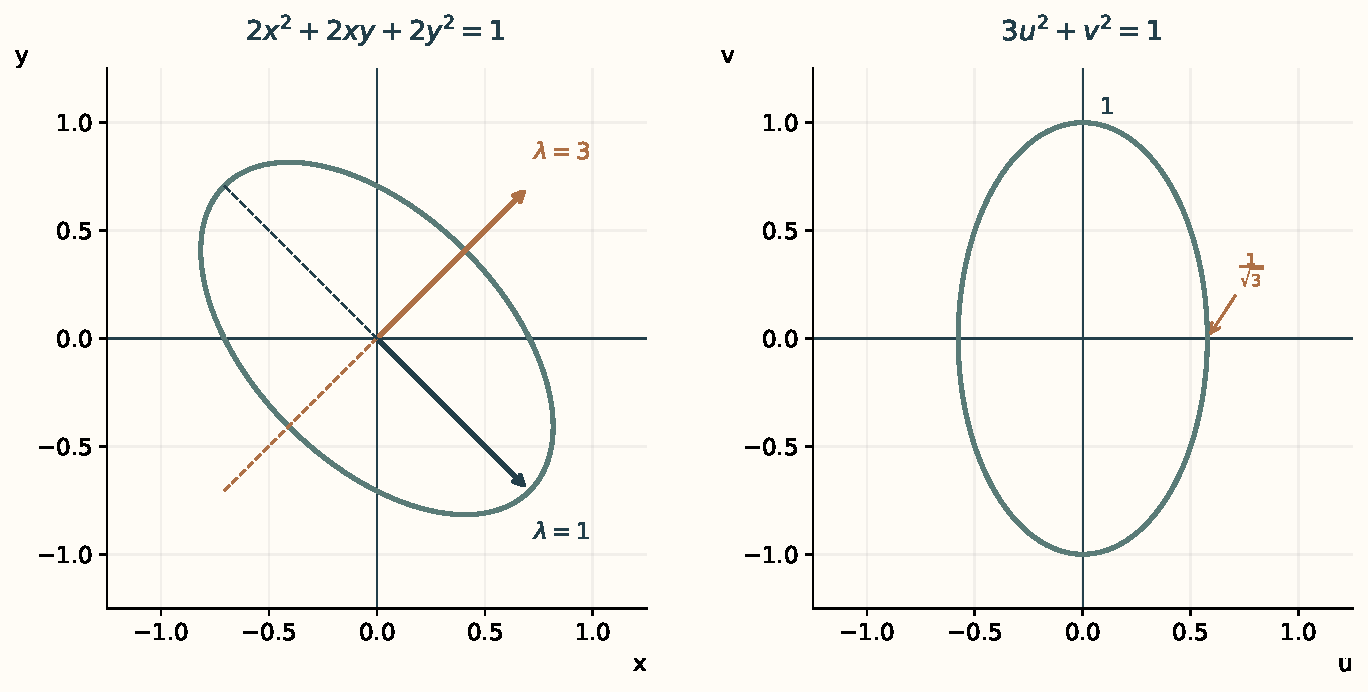
\includegraphics[width=\textwidth,height=.79\textheight,keepaspectratio]{images/atlas-quadratic.pdf}\par\small Главные оси квадратичной формы\end{center}\end{minipage}\par
\Needspace{7\baselineskip}\section*{Задачи}
\begingroup\setlength{\parskip}{2pt}
\noindent\begin{minipage}[t]{\linewidth}\textbf{26.1.} Найди собственные значения и подпространства матрицы \(\begin{pmatrix}2&0\\0&5\end{pmatrix}\).\par\end{minipage}\par
\noindent\begin{minipage}[t]{\linewidth}\textbf{26.2.} Для \(A=\begin{pmatrix}2&1\\1&2\end{pmatrix}\) найди характеристический многочлен и по одному собственному вектору.\par\end{minipage}\par
\noindent\begin{minipage}[t]{\linewidth}\textbf{26.3.} Является ли нулевой вектор собственным вектором? Может ли \(0\) быть собственным значением? Приведи пример.\par\end{minipage}\par
\noindent\begin{minipage}[t]{\linewidth}\textbf{26.4.} Найди все собственные значения \(\begin{pmatrix}0&-1\\1&0\end{pmatrix}\) над \(\mathbb R\) и над \(\mathbb C\).\par\end{minipage}\par
\noindent\begin{minipage}[t]{\linewidth}\textbf{26.5.} Докажи, что если \(Av=\lambda v\), то \(A^mv=\lambda^mv\) для каждого натурального \(m\).\par\end{minipage}\par
\par\addvspace{5pt}\begin{lrbox}{\CatFlowBox}\begin{minipage}[t]{\linewidth}
\setlength{\parskip}{5pt}\setlength{\columnsep}{4.5mm}\setlength{\intextsep}{0pt}
\begin{wrapfigure}[13]{r}{54mm}

\includegraphics[width=54mm,height=58mm,keepaspectratio]{images/unique/art-112.png}
\end{wrapfigure}
\textbf{26.6.} Диагонализируй \(A=\begin{pmatrix}2&1\\1&2\end{pmatrix}\), выбрав ортонормированные столбцы \(P\).\par

\textbf{26.7.} Почему \(J=\begin{pmatrix}1&1\\0&1\end{pmatrix}\) не диагонализируется даже над \(\mathbb C\)?\par

\textbf{26.8.} В заданной модели повторного преобразования \(x_{n+1}=Ax_n\), \(A=\begin{pmatrix}2&1\\1&2\end{pmatrix}\), \(x_0=(1,0)\). Найди \(x_n\).\par

\textbf{26.9.} Для трёхмерного поворота \(A(x,y,z)=(-y,x,z)\) найди неподвижные векторы. Какое собственное значение им соответствует?\par
\par\WFclear\end{minipage}\end{lrbox}%
\ifdim\dimexpr\ht\CatFlowBox+\dp\CatFlowBox\relax<64mm\dp\CatFlowBox=\dimexpr64mm-\ht\CatFlowBox\relax\fi%
\noindent\usebox{\CatFlowBox}\par\addvspace{5pt}

\noindent\begin{minipage}[t]{\linewidth}\textbf{26.10.} Докажи: собственные векторы симметричной действительной матрицы с разными значениями ортогональны.\par\end{minipage}\par
\noindent\begin{minipage}[t]{\linewidth}\textbf{26.11.} Докажи, что диагональная матрица с одним и тем же числом \(c\) на диагонали имеет каждый ненулевой вектор собственным.\par\end{minipage}\par
\noindent\begin{minipage}[t]{\linewidth}\textbf{26.12.}\starmark{} Для \(A=\begin{pmatrix}3&1\\0&2\end{pmatrix}\) найди \(A^n(1,-1)\).\par\end{minipage}\par
\noindent\begin{minipage}[t]{\linewidth}\textbf{26.13.} Запиши симметричную матрицу формы \(3x^2-4xy+5y^2\).\par\end{minipage}\par
\noindent\begin{minipage}[t]{\linewidth}\textbf{26.14.} Определи знак формы \(3x^2-4xy+5y^2\) по критерию положительности.\par\end{minipage}\par
\noindent\begin{minipage}[t]{\linewidth}\textbf{26.15.} Классифицируй формы \(x^2+y^2\), \(-x^2-y^2\), \(x^2-y^2\), \(x^2\).\par\end{minipage}\par
\noindent\begin{minipage}[t]{\linewidth}\textbf{26.16.} Выдели квадрат в \(x^2+4xy+7y^2\) и найди минимум по \(x\) при фиксированном \(y\).\par\end{minipage}\par
\noindent\begin{minipage}[t]{\linewidth}\textbf{26.17.} Найди собственные значения матрицы формы \(2x^2+2xy+2y^2\) и её главные оси.\par\end{minipage}\par
\noindent\begin{minipage}[t]{\linewidth}\textbf{26.18.}\starmark{} В модели энергии \(E=2x^2+2xy+2y^2\) ограничение равно \(x^2+y^2=1\). Найди наименьшее и наибольшее значения энергии.\par\end{minipage}\par
\noindent\begin{minipage}[t]{\linewidth}\textbf{26.19.} При каких действительных \(t\) форма \(x^2+2txy+y^2\) положительно определена?\par\end{minipage}\par
\noindent\begin{minipage}[t]{\linewidth}\textbf{26.20.} Докажи, что \(Q(x,y)=xy\) неопределённа, хотя её матрица обратима.\par\end{minipage}\par
\noindent\begin{minipage}[t]{\linewidth}\textbf{26.21.} Опиши множество \(2x^2+2xy+2y^2=1\) в главных координатах и найди длины его полуосей.\par\end{minipage}\par
\noindent\begin{minipage}[t]{\linewidth}\textbf{26.22.} Докажи: если оба собственных значения симметричной матрицы размера два положительны, то форма положительна на каждом ненулевом векторе.\par\end{minipage}\par
\noindent\begin{minipage}[t]{\linewidth}\textbf{26.23.}\starmark{} Докажи, что форма \(ax^2+2bxy+cy^2\) неотрицательна тогда и только тогда, когда \(a\ge0,c\ge0,ac-b^2\ge0\).\par\end{minipage}\par
\noindent\begin{minipage}[t]{\linewidth}\textbf{26.24.}\starmark{} Построй эскизы уровней \(Q=1\) для \(x^2+y^2\), \(x^2-y^2\), \(x^2\). Какие из них ограничены?\par\end{minipage}\par
\endgroup
